%# -*- coding: utf-8-unix -*-
%======================================================================
% qbook.tex for Qbook Template
%======================================================================
% 双面打印
\documentclass{qbook}
\addbibresource{bib/qbook.bib}  % 导入参考文献数据库
\begin{document}
\pagestyle{empty}
%# -*- coding: utf-8-unix -*-
\thispagestyle{empty}
\begin{tikzpicture}[overlay,remember picture,font=\sffamily\bfseries]
\draw[ultra thick,c4,name path=big arc] ([xshift=-2mm]current page.north) arc(150:285:11)
coordinate[pos=0.225] (x0);
\begin{scope}
\clip ([xshift=-2mm]current page.north) arc(150:285:11) --(current page.north
east);
\fill[c4!50,opacity=0.25] ([xshift=4.55cm]x0) circle (4.55);
\fill[c4!50,opacity=0.25] ([xshift=3.4cm]x0) circle (3.4);
\fill[c4!50,opacity=0.25] ([xshift=2.25cm]x0) circle (2.25);
\draw[ultra thick,c4!50] (x0) arc(-90:30:6.5);
\draw[ultra thick,c4] (x0) arc(90:-30:8.75);
\draw[ultra thick,c4!50,name path=arc1] (x0) arc(90:-90:4.675);
\draw[ultra thick,c4!50] (x0) arc(90:-90:2.875);
\path[name intersections={of=big arc and arc1,by=x1}];
\draw[ultra thick,c4,name path=arc2] (x1) arc(135:-20:4.75);
\draw[ultra thick,c4!50] (x1) arc(135:-20:8.75);
\path[name intersections={of=big arc and arc2,by={aux,x2}}];
\draw[ultra thick,c4!50] (x2) arc(180:50:2.25);
\end{scope} 
\path[decoration={text along path,text color=c4,
	raise = -2.8ex,
	text  along path,
	text = {|\sffamily\bfseries|\today},
	text align = center,
},
decorate
] ([xshift=-2mm]current page.north) arc(150:245:11);
%
\begin{scope}
\path[clip,postaction={fill=c3}]
([xshift=2cm,yshift=-8cm]current page.center) rectangle ++ (4.2,7.7);
\fill[c2] ([xshift=0.5cm,yshift=-8cm]current page.center)
([xshift=0.5cm,yshift=-8cm]current page.center)  arc(180:60:2)
|- ++ (-3,6) --cycle;
\draw[ultra thick,c4] ([xshift=-1.5cm,yshift=-8cm]current page.center) 
arc(180:0:2);
\draw[ultra thick,c4] ([xshift=0.5cm,yshift=-8cm]current page.center) 
arc(180:0:2);
\draw[ultra thick,c4] ([xshift=2.5cm,yshift=-8cm]current page.center) 
arc(180:0:2);
\draw[ultra thick,c4] ([xshift=4.5cm,yshift=-8cm]current page.center) 
arc(180:0:2);
\fill[red] ([xshift=2.5cm,yshift=-8cm]current page.center) +(60:2) circle(1.5mm);
\node[text=c5!80!black] at ([xshift=4.7cm,yshift=-5.2cm]current page.center) {$\rho:=\dfrac{1+\sqrt{-3}}{2}$};
\end{scope}
%
\fill[c1] ([xshift=2cm,yshift=-8cm]current page.center) rectangle ++ (-13.7,7.7);
\node[text=white,anchor=west,scale=4,inner sep=0pt] at
([xshift=-10.55cm,yshift=-3cm]current page.center) {$\mathbb{ Q }$-book 书籍模板};
\node[text=white,anchor=west,scale=2,inner sep=0pt] at
([xshift=-4.5cm,yshift=-5.5cm]current page.center) {333 \quad 制作};
\end{tikzpicture}  % 载入封面
\begin{center}
	\Large{\sffamily\bfseries\heiti Version 2.00} \\ \vspace{2em}
	\Large{\sffamily\bfseries\heiti 编译日期: \today} \\ \vspace{1em}
	\Large{\sffamily\bfseries\heiti 任何建议及错误信息请发送至邮箱} \\
	\texttt{jey74165@163.com}
\end{center} 
\vfill
\vspace{30em}
\begin{tabular*}{\textwidth}{ccc}
	\includegraphics{figure/by-nc.eps}
	& \begin{minipage}[b]{0.6\textwidth}
		\small\sffamily
		本作品采用知识共享 署名-非商业性使用 4.0 国际 许可协议进行许可. 访问\url{http://creativecommons.org/licenses/by-nc/4.0/  }查看该许可协议.
	\end{minipage}
\end{tabular*}  
\thispagestyle{empty}
\frontmatter  % 对前言和概览用罗马数字作为页码
\pagestyle{empty}
%%%%%%%%%%%%%%%%%%%%%%preface.tex%%%%%%%%%%%%%%%%%%%%%%%%%%%%%%%%%%%%%%%%%
% sample preface
%
% Use this file as a template for your own input.
%
%%%%%%%%%%%%%%%%%%%%%%%% Springer %%%%%%%%%%%%%%%%%%%%%%%%%%

\preface

%% Please write your preface here
Use the template \emph{preface.tex} together with the Springer document class SVMono (monograph-type books) or SVMult (edited books) to style your preface in the Springer layout.

A preface\index{preface} is a book's preliminary statement, usually written by the \textit{author or editor} of a work, which states its origin, scope, purpose, plan, and intended audience, and which sometimes includes afterthoughts and acknowledgments of assistance. 

When written by a person other than the author, it is called a foreword. The preface or foreword is distinct from the introduction, which deals with the subject of the work.

Customarily \textit{acknowledgments} are included as last part of the preface.
 

\vspace{\baselineskip}
\begin{flushright}\noindent
Place(s),\hfill {\it Firstname  Surname}\\
month year\hfill {\it Firstname  Surname}\\
\end{flushright}



\pagestyle{empty}
\tableofcontents
\cleardoublepage
%# -*- coding: utf-8-unix -*-
\begin{overview}
\thispagestyle{empty}
在2018年3月底,翻译\footnote{这个模板原本是用于一项书籍翻译计划的,关注我公众号的读者对此有所了解。然而由于版权原因,该译本无法公开分享。}进度已过大半,于是开始着手进行\LaTeX 排版。在此之前我对\LaTeX 的了解微乎其微,甚至第一次安装TexLive就出了问题,不得不重新安装。也是借着给这个译本排版的机会,才逐渐熟悉了这一软件的使用方法。

如大家所见,模板的封面和扉页设计均高仿\footnote{李老师的书籍源码尚未公开,此为仿作。}自李文威老师《模形式初步》一书,并已得到李老师的使用许可;定理和定义环境则取材自网上流传的Elegantbook模版。我也从这一以模仿为主的学习过程中,对\LaTeX 有了更深入的了解。

本模板命名为$\mathbb{ Q }$-book,谐音自cubic一词。由于是一个菜鸟的作品,自然还有许多瑕疵,对此模板的错误和不足之处还请各位多多包涵。

\end{overview}
 
\mainmatter	  % 对正文用阿拉伯数字作为页码
%======================================================================
% 正文内容
\pagestyle{fancy}
\setcounter{page}{0}
%# -*- coding: utf-8-unix -*-
%%==================================================
\chapter{这是什么?}

这是$\mathbb{ Q}$-book \LaTeX 书籍模板,当前版本为 \version 。

这份模板主要基于上海交大的学位论文模板
\footnote{\url{https://github.com/sjtug/SJTUThesis}}修改得到
,结合少量个人审美喜好,重新定制了定义、定理等环境。由于这个模板本是用于一项书籍翻译计划,因此其中的一些环境,例如“观察”、“规则”、“关键点”等,读者可能用不到,可以根据自己的需求适当修改。

你也可以通过邮箱\texttt{jey74165@163.com}给我发邮件反映遇到的问题。不过作者水平有限,或许有些问题也无法解答,还请见谅。

\section{文档说明}

\subsection{准备工作}

要想灵活使用、魔改这个模板来撰写自己的书籍,需要对\emph{TeX系统}有一定的了解,也需要掌握基本的\emph{TeX技能}。

\begin{itemize}[noitemsep,topsep=0pt,parsep=0pt,partopsep=0pt]
	\item {\TeX}系统:所使用的{\TeX}系统要支持 \XeTeX 引擎,且带有ctex 2.x宏包。一般来说,只要安装了的\emph{完整}TeXLive或MacTeX发行版就不会出现问题。
	\item TeX技能:尽管提供了对模板的必要说明,但这并不是一份“ \LaTeX 入门文档”。用户应当有一定的\LaTeX 使用经验。
\end{itemize}

\subsection{字体与选项}

$\mathbb{ Q }$-book暂不提供可选项,直接用命令\verb|\documentclass{qbook}|载入即可。如有需要,用户可以根据自己的需求进行相关的添加或修改。

本模板所使用的字体仅为宋体,{\kaishu{楷体}}和{\heiti{黑体}}等自带字体,用户不会在字体问题上折腾太多精力。

\subsection{编译方式}

最简单的办法是直接双击模板文件夹中的compile.bat文件,在命令行模式下编译;当然使用你配置好的Tex编辑器也是可以的。编译失败时,可以尝试手动逐次编译,定位故障。
\begin{lstlisting}[basicstyle=\small\ttfamily, caption={手动逐次编译}, numbers=none]
xelatex -no-pdf qbook
biber --debug qbook
xelatex qbook
xelatex qbook
\end{lstlisting}

\section{模板文件介绍}

本节介绍$\mathbb{ Q }$-book模板中主要文件和目录的功能。

\subsection{格式控制文件}

格式控制文件控制着书籍的表现形式,包括以下两个文件
\begin{itemize}[noitemsep,topsep=0pt,parsep=0pt,partopsep=0pt]
	\item qbook.cfg
	\item qbook.cls
\end{itemize}
其中,“cfg”和“cls”为文件格式。

\subsection{主文件}

主文件qbook.tex的作用就是将你分散在多个文件中的章节重新“拼合”成一本完整的书。
当我们用\LaTeX 写书时,肯定不希望一直在同一页面码字,那样会显得非常臃肿,而且不便于以后的修改和查找。所以在使用本模板的时候,你的章节内容和素材会被“拆散”为各个部分,例如前言、概览、各章节及参考文献等。
在qbook.tex中通过\verb|\include{xxx}|命令将各个部分包含进来,从而形成一本结构完整的书籍。

\subsection{各部分源文件}

被“拆散”的各个部分的源文件存放于tex文件夹中,是论文的主体,以“章”为单位划分,其中包括:

\begin{itemize}[noitemsep,topsep=0pt,parsep=0pt,partopsep=0pt]
	\item cover.tex——用于绘制封面。
	\item preface.tex——前言。
	\item overview.tex——概览。
	\item chapter(xxx).tex——各章主体内容。
	\item 参考文献列表由bibtex插入,不作为一个单独的文件。
\end{itemize}

\subsection{图片存放}

figure文件夹放置了需要插入文档中的图片文件(支持PNG/JPG/PDF/EPS格式的图片)。
在qbook.cls中已经使用\verb|\graphicspath|命令定义了图片存储的顶层目录,所以在插入图片时,图片路径的顶层目录名“figure”可省略。

\subsection{参考文献数据库}

目前参考文件数据库目录只存放一个参考文件数据库qbook.bib。
关于参考文献引用,可参考第\ref{chap2}章中的例子。

%# -*- coding: utf-8-unix -*-
%%==================================================

\chapter{写作示例}
\label{chap2}

\section{列表环境}

\subsection{无序列表}

以下是一个无序列表的例子,列表的每个条目单独分段。

\begin{itemize}
	\item 这是一个无序列表。
	\item 这是一个无序列表。
	\item 这是一个无序列表。
\end{itemize}

使用\verb+itemize*+环境可以创建行内无序列表。
\begin{itemize*}
	\item 这是一个无序列表
	\item 这是一个无序列表
	\item 这是一个无序列表
\end{itemize*}
行内无序列表条目不单独分段,所有内容直接插入在原文的段落中。

\subsection{有序列表}

使用环境\verb+enumerate+和\verb+enumerate*+创建有序列表,
使用方法无序列表类似。
\begin{enumerate}
	\item 这是一个有序列表。
	\item 这是一个有序列表。
	\item 这是一个有序列表。
\end{enumerate}

使用\verb+enumerate*+环境可以创建行内有序列表。
\begin{enumerate*}
	\item 这是一个默认有序列表
	\item 这是一个默认有序列表
	\item 这是一个默认有序列表
\end{enumerate*}
行内有序列表条目不单独分段,所有内容直接插入在原文的段落中。

\subsection{描述列表}
使用环境\verb+description+可创建带有主题词的列表,条目语法是\verb+\item[主题] 内容+。
\begin{description}
	\item[主题一] 详细内容
	\item[主题二] 详细内容
	\item[主题三] 详细内容 \ldots
\end{description}

\section{数学排版}

\subsection{公式排版}

这里有举一个长公式排版的例子,来自\href{http://www.tex.ac.uk/tex-archive/info/math/voss/mathmode/Mathmode.pdf}{《Math mode》}:

\begin {multline}
\frac {1}{2}\Delta (f_{ij}f^{ij})=
2\left (\sum _{i<j}\chi _{ij}(\sigma _{i}-
\sigma _{j}) ^{2}+ f^{ij}\nabla _{j}\nabla _{i}(\Delta f)+\right .\\
\left .+\nabla _{k}f_{ij}\nabla ^{k}f^{ij}+
f^{ij}f^{k}\left [2\nabla _{i}R_{jk}-
\nabla _{k}R_{ij}\right ]\vphantom {\sum _{i<j}}\right )
\end{multline}

\subsection{SI单位}

使用\verb+siunitx+宏包可以方便地输入SI单位制单位,例如\verb+\SI{5}{\um}+可以得到\SI{5}{\um}。

\subsection{定理环境}

在这个模板中,定义了如下几个环境
remark(注),mythm(定理),myprop(性质),mydef(定义),example(例)。
amsmath还提供了一个proof(证明)的环境。
我们举例说明它们的用法。

注环境
\begin{remark}
	存在事先给定的一系列基本操作,并且这些基本操作永远不会改变。
\end{remark}
\begin{remark}
	每个操作都可逆。
	\label{o1.2}
\end{remark}
\begin{remark}
	每一个操作都是确定性的。
\end{remark}
\begin{remark}
	各个操作可以按任何顺序组合。
\end{remark}

性质环境
\begin{myprop}{}{}
	存在一些预先定义的永不发生改变的作用(action)。
\end{myprop}

\begin{myprop}{}{}
	每一个作用都可逆。
\end{myprop}

\begin{myprop}{}{}
	每个作用都是确定性的。
\end{myprop}

\begin{myprop}{}{}
	任意的一系列连续的作用仍然是一个作用。
\end{myprop}

例子环境
\begin{example}
	天地玄黄,宇宙洪荒。
	\soln
	
	日月盈仄,辰宿列张。
\end{example}

定义环境
\begin{mydef}{域}{1}
	设$S$为一个非空集合,其上有“加法”(记作$+$)与“乘法”(记作$\cdot$)两种代数运算. 若满足以下条件,则称$(S,+,\cdot)$构成一个域(field).
	\begin{itemize}
		\item[(1)] $(S,+)$构成一个交换群.
		\item[(2)] 若记$S^{*}=S-\{0\}$,其中$0$为群$(S,+)$中的单位元,则$(S^{*},\cdot)$也构成一个交换群.
		\item[(3)] 乘法对加法有分配律:$a ( b + c ) = a b + a c$.
	\end{itemize}
\end{mydef}

关键点环境
\begin{keypoint}
	伽罗瓦理论在分析从有理数域$\mathbb{ Q }$扩张到新的域的运算或操作时很有用。我们的大问题可以用伽罗瓦理论来回答,数学中其他的一些历史问题也同样可以用伽罗瓦理论来解答。
\end{keypoint}

定理环境
\begin{mythm}{望远镜公式}{2}
	$\left[\mathbb{Q}(a, b) : \mathbb{Q}\right]=\left[\mathbb{Q}(a, b) : \mathbb{Q}(a)\right]\left[\mathbb{Q}(a) : \mathbb{Q}\right] $
\end{mythm}

\begin{proof}
	
	\rthm{thm:2}告诉我们,对任意$s\in S$,均有$\lvert Orb(s)\rvert \cdot \lvert Stab(s)\rvert=\lvert G\rvert=p$. 于是$\lvert Orb(s)\rvert $整除$p$,这里$p$是一个素数。从而$\lvert Orb(s)\rvert $等于1或$p$,也就是说,\textbf{所有轨道的大小要么为1,要么为$p$}. 于是整个集合$S$就被划分为两部分,一部分是大小为1的轨道,另一部分是大小为$p$的轨道,如图9.4所示。
	
	假设大小为1的轨道有$m$个,大小为$p$的轨道有$n$个,则有
 \begin{equation}
		m+p\cdot n=\lvert S\rvert 
 \end{equation}
	注意到\rdef{def:1},\textbf{那些$\lvert Orb(s)\rvert =1$的元素$s$即为稳定元},这就表明有$m$个稳定元。从上式立刻看出$\lvert S \rvert \equiv  m\; (\bmod\; p)$.	
\end{proof}

\section{表格}

这一节给出的是一些表格的例子,如表\ref{tab1}所示。

\begin{table}[!hpb]
	\centering
	\bicaption[指向一个表格的表目录索引]
	{一个颇为标准的三线表格\footnotemark[1]}
	{A Table}
	\label{tab1}
	\begin{tabular}{@{}llr@{}} \toprule
		\multicolumn{2}{c}{Item} \\ \cmidrule(r){1-2}
		Animal & Description & Price (\$)\\ \midrule
		Gnat & per gram & 13.65 \\
		& each & 0.01 \\
		Gnu & stuffed & 92.50 \\
		Emu & stuffed & 33.33 \\
		Armadillo & frozen & 8.99 \\ \bottomrule
	\end{tabular}
\end{table}
\footnotetext[1]{这个例子来自\href{http://www.ctan.org/tex-archive/macros/latex/contrib/booktabs/booktabs.pdf}{《Publication quality tables in LATEX》}(booktabs宏包的文档)。这也是一个在表格中使用脚注的例子,请留意与threeparttable实现的效果有何不同。}

下面一个是一个更复杂的表格,用threeparttable实现带有脚注的表格,如表\ref{tab2}。

\begin{table}[!htpb]
	\bicaption[出现在表目录的标题]
	{一个带有脚注的表格的例子}
	{A Table with footnotes}
	\label{tab2}
	\centering
	\begin{threeparttable}[b]
		\begin{tabular}{ccd{4}cccc}
			\toprule
			\multirow{2}{6mm}{total}&\multicolumn{2}{c}{20\tnote{1}} & \multicolumn{2}{c}{40} &  \multicolumn{2}{c}{60}\\
			\cmidrule(lr){2-3}\cmidrule(lr){4-5}\cmidrule(lr){6-7}
			&www & \multicolumn{1}{c}{k} & www & k & www & k \\ % 使用说明符 d 的列会自动进入数学模式,使用 \multicolumn 对文字表头做特殊处理
			\midrule
			&$\underset{(2.12)}{4.22}$ & 120.0140\tnote{2} & 333.15 & 0.0411 & 444.99 & 0.1387 \\
			&168.6123 & 10.86 & 255.37 & 0.0353 & 376.14 & 0.1058 \\
			&6.761    & 0.007 & 235.37 & 0.0267 & 348.66 & 0.1010 \\
			\bottomrule
		\end{tabular}
		\begin{tablenotes}
			\item [1] the first note.% or \item [a]
			\item [2] the second note.% or \item [b]
		\end{tablenotes}
	\end{threeparttable}
\end{table}

\section{插入图片}

\XeTeX 可以很方便地插入PDF、PNG、JPG格式的图片。插入PNG/JPG的例子如\ref{fig1}所示。
这两个水平并列放置的图共享一个“图标题”(table caption),没有各自的小标题。

\begin{figure}[!htp]
\centering

\includegraphics[width=4cm]{example/by-nc.png}
\hspace{1cm}
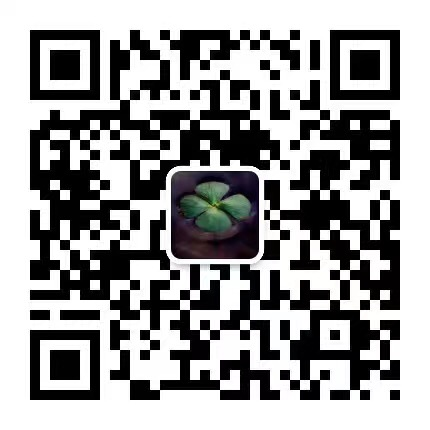
\includegraphics[width=4cm]{example/gzh.jpg}
\bicaption{中文题图}
{English caption}
\label{fig1}
\end{figure}

这里还有插入EPS图像和PDF图像的例子,如图\ref{fig2}和图\ref{fig3}。这里将EPS和PDF图片作为子图插入,每个子图有自己的小标题。子图标题使用subcaption宏包添加。

\begin{figure}[!htp]
\centering
\subcaptionbox{EPS 图像\label{fig2}}[3cm] %标题的长度,超过则会换行,如下一个小图。
{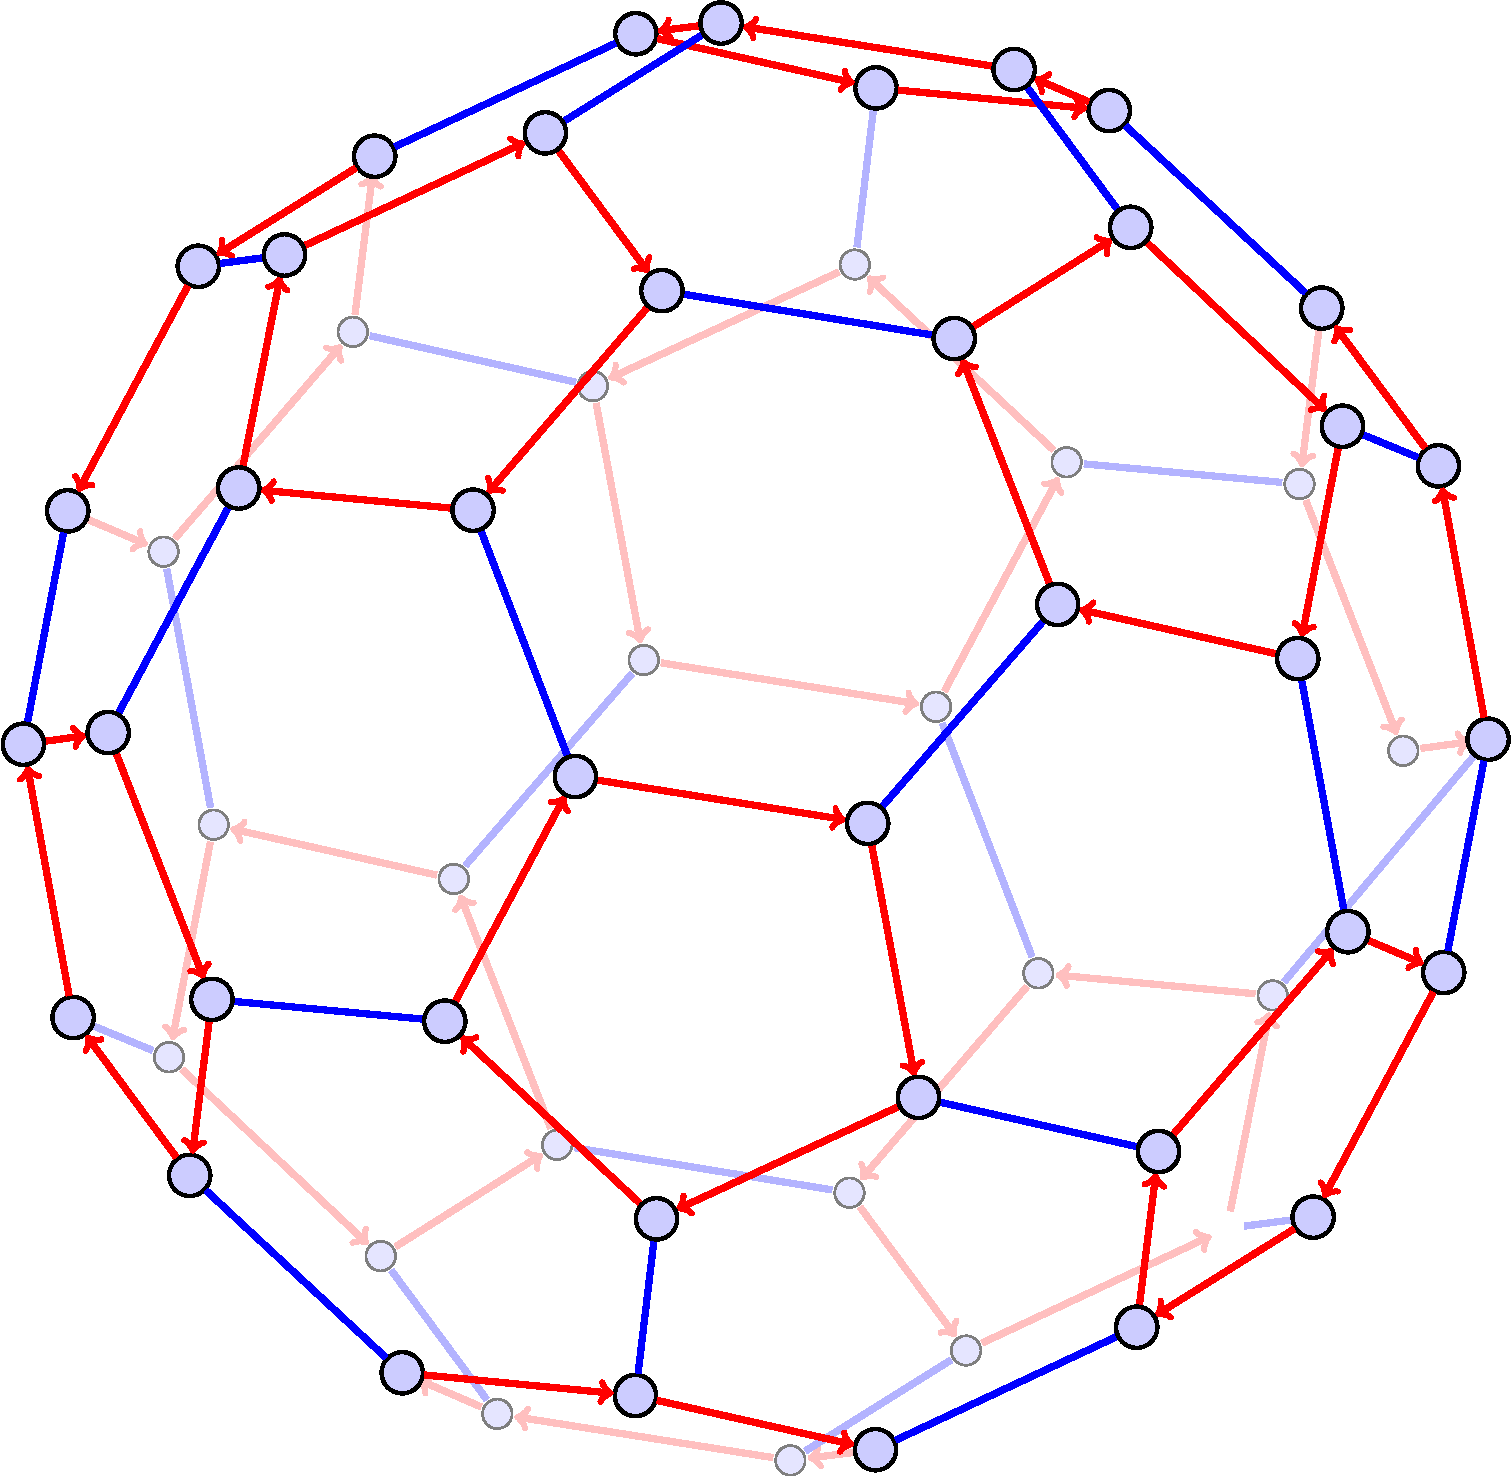
\includegraphics[height=2.5cm]{example/m2.pdf}}
\hspace{4em}
\subcaptionbox{PDF 图像,注意这个图略矮些。如果标题很长的话,它会自动换行\label{fig3}}
{	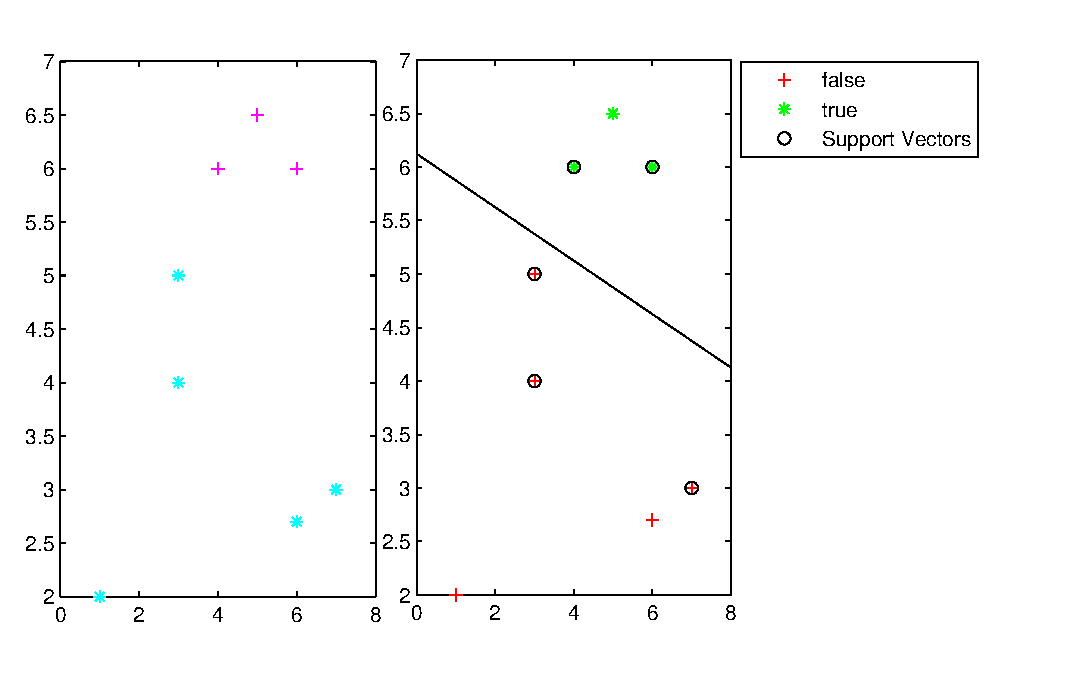
\includegraphics[scale=0.5]{example/figep.eps}}
\bicaption{插入eps和pdf的例子(使用 subcaptionbox 方式)}{An EPS and PDF demo with subcaptionbox}
\label{fig4}
\end{figure}




\section{插入代码}

这里给一个使用listings宏包插入源代码的例子:
\begin{lstlisting}[language={C}, caption={一段C源代码}]
#include <stdio.h>
#include <unistd.h>
#include <sys/types.h>
#include <sys/wait.h>

int main() {
pid_t pid;

switch ((pid = fork())) {
case -1:
printf("fork failed\n");
break;
case 0:
/* child calls exec */
execl("/bin/ls", "ls", "-l", (char*)0);
printf("execl failed\n");
break;
default:
/* parent uses wait to suspend execution until child finishes */
wait((int*)0);
printf("is completed\n");
break;
}

return 0;
}
\end{lstlisting}


\section{参考文献管理}
\label{sec2.5}
\LaTeX 具有将参考文献内容和表现形式分开管理的能力,涉及三个要素:参考文献数据库、参考文献引用格式、在正文中引用参考文献。
这样的流程需要多次编译:
\begin{enumerate}[noitemsep,topsep=0pt,parsep=0pt,partopsep=0pt]
\item 用户将论文中需要引用的参考文献条目,录入纯文本数据库文件(bib文件)。
\item 调用xelatex对论文模板做第一次编译,扫描文中引用的参考文献,生成参考文献入口文件(aux)文件。
\item 调用bibtex,以参考文献格式和入口文件为输入,生成格式化以后的参考文献条目文件(bib)。
\item 再次调用xelatex编译模板,将格式化以后的参考文献条目插入正文。
\end{enumerate}

参考文献数据库(thesis.bib)的条目,可以从Google Scholar搜索引擎\footnote{\url{https://scholar.google.com}}、CiteSeerX搜索引擎\footnote{\url{http://citeseerx.ist.psu.edu}}中查找,文献管理软件Papers\footnote{\url{http://papersapp.com}}、Mendeley\footnote{\url{http://www.mendeley.com}}、JabRef\footnote{\url{http://jabref.sourceforge.net}}也能够输出条目信息。

下面是在Google Scholar上搜索到的一条文献信息,格式是纯文本:

\begin{lstlisting}[caption={从Google Scholar找到的参考文献条目}, label=googlescholar, escapeinside="", numbers=none]
@phdthesis{"白2008信用风险传染模型和信用衍生品的定价",
title={"信用风险传染模型和信用衍生品的定价"},
author={"白云芬"},
year={2008},
school={"上海交通大学"}
} 
\end{lstlisting}

推荐修改后在bib文件中的内容为:

\begin{lstlisting}[caption={修改后的参考文献条目}, label=itemok, escapeinside="", numbers=none]
@phdthesis{bai2008,
title={"信用风险传染模型和信用衍生品的定价"},
author={"白云芬"},
date={2008},
address={"上海"},
school={"上海交通大学"}
} 
\end{lstlisting}

参考文献的引用:
\begin{itemize}
\item 参考文献在正文中被引用,使用命令\verb+\cite{key}+,如\cite{M91}。
\item 参考文献未引用但仍希望列在书末的参考文献中,使用命令\verb+\nocite{key}+,如\verb+\nocite{WI64,G03,D01,JS03}+.
\end{itemize}
\nocite{WI64,G03,D01,JS03}
%# -*- coding: utf-8-unix -*-


%# -*- coding: utf-8-unix -*-
%%==================================================

\include{tex/chapter5}
\include{tex/chapter6}
\include{tex/chapter7}



\include{tex/chapter9}
\include{tex/chapter10}
\backmatter	
%======================================================================
% 打印参考文献
\printbibliography[heading=bibintoc]
\makeatletter
\makeatother
\end{document}